\documentclass[10pt]{article}
\usepackage{graphicx}
\usepackage{hyperref}
\usepackage[ngerman]{babel}
\usepackage{siunitx}
\sisetup{
  locale = DE ,
  per-mode = symbol  % whether it should print "/" or "^-1"
}

\usepackage[margin=2cm]{geometry}
\usepackage{multicol}
\usepackage{nicefrac}
\usepackage{todonotes}
\usepackage{amsmath}
\usepackage{amssymb}

% \usepackage{pdflscape}
% \usepackage{pdfpages}
% \usepackage{epstopdf}
% \epstopdfDeclareGraphicsRule{.tiff}{png}{.png}{convert -density 180 #1 \OutputFile}
% \AppendGraphicsExtensions{.tiff}


\author{Team 03}
\title{Abgabe 1 Autonomes Fahren}
\begin{document}
\maketitle
\tableofcontents

\section{Masse}
    \subsection{gesamtes Auto}
    Die Waage kann nur eine Masse bis \SI{2}{\kilogram} messen, deshalb wurde wie folgt ein Gesamtgewicht von \SI{2261,13}{\gram} errechnet:
    \begin{multicols}{3}
    \begin{itemize}
        \item Akku: $\SI{404,32}{\gram}$
        \item Fahrzeug: $\SI{1841,36}{\gram}$
        \item Akkuhalterung: $\SI{15,45}{\gram}$
    \end{itemize}
    \end{multicols}

    \subsection{Einzelmessungen}
    Für spätere Berechnungen und zur Sicherheit wurde eine Messung der enthaltenen Einzelteile (soweit möglich) durchgeführt. Dies hat folgende Massen ergeben:
    \begin{multicols}{3}
    \begin{itemize}
        \item Einzelnes Rad: $\SI{37,35}{\gram}$
        \item 4 Räder: $\SI{149,74}{\gram}$
        \item Motor: $\SI{181,87}{\gram}$
        \item Raspberry Pi: $\SI{50,18}{\gram}$
        \item IBT\_2 (blau): $\SI{65,99}{\gram}$
        \item Verschaltung: $\SI{48,13}{\gram}$
        \item Chassis: $\SI{762,99}{\gram}$
        \item Kameraaufhängung: $\SI{147,05}{\gram}$
        \item Grundplatte für Technik: $\SI{227,32}{\gram}$
        \item Servomotor: $\SI{63,81}{\gram}$
        \item Kamera: $\SI{3,38}{\gram}$
        \item Schalter: NaN
        \item div Schrauben: $\SI{3,73}{\gram}$
        \item div Schrauben: $\SI{4,14}{\gram}$
        \item div Schrauben (Verbindung vom Chassis zur Technik): $\SI{38,11}{\gram}$
        \item IMU (beschleunigungssensor): NaN
        \item Kabel zwischen blauer Platine und Steuerungseinheit: $\SI{7,12}{\gram}$
        \item Sicherung: $\SI{34,47}{\gram}$
    \end{itemize}
    \end{multicols}

\section{Schwerpunkt}
    Der wahre Schwerpunkt kann nicht ermittelt werden, dieser liegt im Inneren der Karosserie.
    Wir haben die Schwerpunktslage bezogen auf die Grundfläche auf zwei verschieden Arten ermittelt:
    \begin{itemize}
    \item Zum einen wurde das Gewicht mit Federwagen in $X$-Richtung gemessen, Werte waren vorne $\SI{7,1}{\newton}$ und hinten $\SI{14,5}{\newton}$ bei einem Abstand zwischen den Messpunkten von $\SI{31,5}{\cm}$. Dies führt zu einer Schwerpunktslage von $31,5 \cdot \nicefrac{7,1}{7,1+14,5} \approx 10,354$ gegenüber dem hinteren Messpunkt und einer Schwerpunktslage von $31,5 \cdot \nicefrac{14,5}{7,1+14,5} \approx 21,146$ gegenüber dem vorderen Messpunkt.
    \item Weiter haben wir eine Messung mit Waage durchgeführt. Hierbei wurde eine Achse aufgelegt und gemessen, während die andere in Gleichgewichtslage fix gehalten wurde. Gemessen wurden vorne $\SI{907,4}{\gram}$ und hinten $\SI{1305,3}{\gram}$ bei einem Abstand zwischen den Achsen (Messpunkten) von \SI{28,5}{\cm}. Dies führt zu einer Schwerpunktslage von $28,5\cdot\nicefrac{907,4}{907,4+1305,3} \approx 11,687$ gegenüber dem hinteren Messpunkt beziehungsweise einer Schwerpunktslage von $28,5\cdot\nicefrac{1305,3}{907,4+1305,3} \approx 17,608$ gegenüber dem vorderen Messpunkt.
    \end{itemize}

    Hierbei sind wir davon ausgegangen, dass der Schwerpunkt in $Y$-Richtung (seitlich) zu vernachlässigen sei. Zwei Messungen mit Federwagen haben folgende Ergebnisse geliefert:
    \begin{itemize}
        \item links \SI{11,1}{\newton} sowie rechts \SI{9}{\newton}
        \item links \SI{10}{\newton} sowie rechts \SI{10,5}{\newton}
    \end{itemize}

    Die Unterschiede sind hier auf Messfehler zurückzuführen, im Mittel ist die Schwerpunktslage in diese Richtung zu vernachlässigen und nur wie oben beschrieben in $X$-Richtung zu betrachten.
    Auch in $X$-Richtung traten verschiedene Unterschiede auf, im Mittel lässt sich aber (wie erwartet) sagen dass sich der Schwerpunkt etwa im hinteren Drittel auf Höhe des Motors befindet.

\section{Trägheit}
Um die Trägheit zu errechnen, wurde ein Versuch an einem Pendel durchgeführt.
Das an einer Lichtschranke anliegende Signal, sobald das Pendel diese durchläuft, wurde in einem Oszilloskop\footnote{MDO3000 series, compare \url{~/Downloads/MDO3000-Oscilloscope-User-Manual.pdf}} als CSV Datei exportiert und in den Abbildungen \ref{fig:AufhaengungohneGummi}, \ref{fig:AufhaengungmitGummi} und \ref{fig:AufhaengungmitGummiundAuto} analysiert.
Hier sieht man, dass für die Aufhängung eine mittlere Periodendauer von zwischen $\SI{1,44}{\second}$ und $\SI{1,45}{\second}$ vorliegt, während diese für das Auto $\SI{1,37}{\second}$ beträgt.

Wir haben folgende Gleichungen (mit $T=\frac{2\pi}{\omega} = 2\pi\sqrt{\frac{I}{mgl}}$ Periodendauer, $I$ Trägheitsmoment, $\omega$ Kreisfrequenz, $m$ Masse, $g$ Erdbeschleunigung und $l$ Länge des Pendels) zugrunde gelegt:
\begin{eqnarray}
    &\ddot{x}(t) + \omega^2x(t)& = 0 \\
    \Leftrightarrow &\ddot{\alpha}(t) + \frac{mgl}{I}\alpha(t)& = 0 \\
    \Leftrightarrow &I\ddot{\alpha} + \alpha mgl& = 0 \\
\end{eqnarray}


\todo[inline]{ausformulieren}Steiner anteil:

$I_{\text{Car}}=(t_{\text{auto}}^2/(2pi)^2\cdot 9,81\cdot m_{\text{gesamt}}\cdot l_{\text{ges}}-l_{car}^2\cdot m_c-l_{\text{gerüst}}^2\cdot (m_p+m_g)-I_{\text{gerüst}}$

Einsetzen ergibt (wenn $I_{\text{gerüst}} = 0,0625$ und $L_{\text{car}} = 0,385$ angenommen wird) $I_{\text{Car}} = 0,0274$. Andere gruppen haben hier bis zu $0,04$ errechnet / gemessen. Dies resultiert möglicherweise aus der Annahme $L_{\text{car}}$, durch die fehlende Berücksichtigung des Schwerpunkts.


\begin{figure}[htbp]
    \centering
    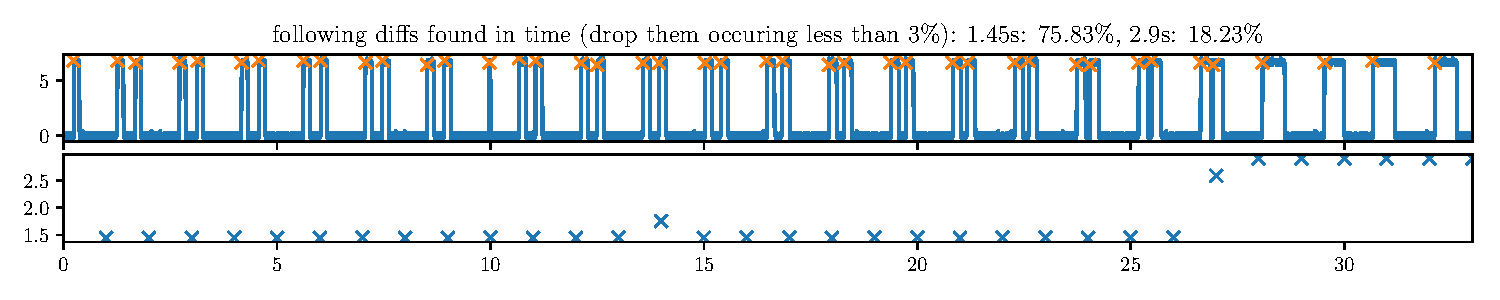
\includegraphics[width=\textwidth]{figures/AufhaengungohneGummi.pdf}
    \caption{Aufhängung ohne fixierende Gummibänder}\label{fig:AufhaengungohneGummi}
\end{figure}
\begin{figure}[htbp]
    \centering
    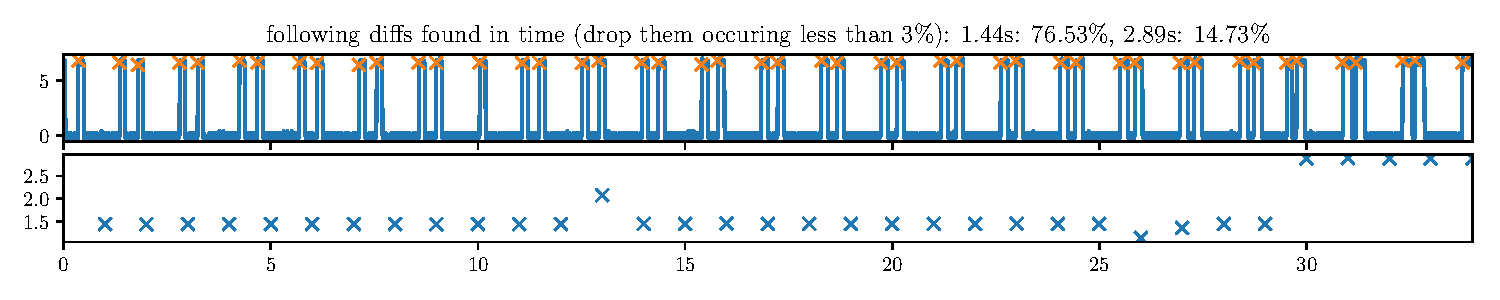
\includegraphics[width=\textwidth]{figures/AufhaengungmitGummi.pdf}
    \caption{Aufhängung mit Halterung}\label{fig:AufhaengungmitGummi}
\end{figure}
\begin{figure}[htbp]
    \centering
    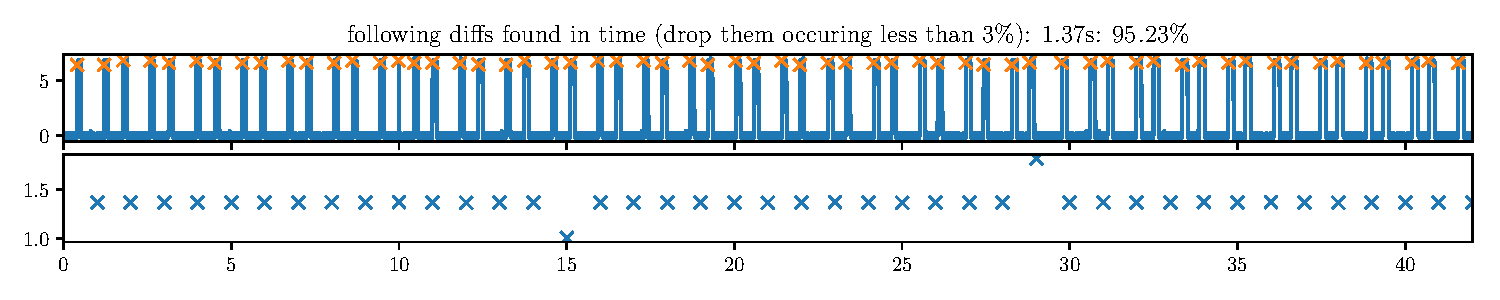
\includegraphics[width=\textwidth]{figures/AufhaengungmitGummiundAuto.pdf}
    \caption{Aufhängung mit befestigtem Auto}\label{fig:AufhaengungmitGummiundAuto}
\end{figure}


\section{Radius}
maximaler Einschlagwinkel (300), 133,7m


\section{dynamischer radius}
\begin{itemize}
    \item 1. run 500
    \item 2. run 1000
    \item 3. run 2000
\end{itemize}


\section{Motor-Kennlinie} % (fold)
\label{sec:motor_kennlinie}
In der Motorkennlinie beobachteten wir lineares Verhalten, der Eingang wird also nur skaliert.
Der Motor arbeitet mit einem Eingang zwischen $0$ und $4095$ Einheiten.
Beim Aufnehmen der Motorkennlinie mit Python beginnt diese erst bei $1000$ Einheiten;
erst dort beginnt das Auto, sich zu bewegen.
Andere Gruppen beobachteten allerdings ein nicht-lineares Verhalten mit fallender Steigung und nahezu logarithmisch verlaufender Kennlinie.
Zudem liegt die durch uns gemessene Maximalgeschwindigkeit von $4000$ Einheiten unter Vergleichswerten anderer Teams.
Die Problematik ist uns bewusst und könnte aus unterschiedlicher Modellierung und der Steuerung der Autos resultieren.
Vor weiterer Modellierung werden wir diesen Aspekt gemeinsam mit anderen Teams weiter untersuchen.

% section motor_kennlinie (end)






\end{document}
